\documentclass[11pt, a4paper]{article}

\usepackage{amsmath, amssymb, titling}
\usepackage[margin=2.5cm]{geometry}
\usepackage[colorlinks=true, linkcolor=black, urlcolor=black, citecolor=black]{hyperref}
\usepackage{graphicx}
\usepackage{caption}
\usepackage{subcaption}
\usepackage{float}
\usepackage{cancel}
\usepackage{fancyhdr, lastpage}
\usepackage{fourier-orns}
\usepackage{xcolor}
\usepackage{nomencl}
\usepackage{etoolbox}
\makenomenclature

\setlength{\headheight}{18.2pt}
\setlength{\nomlabelwidth}{1.5cm}

\renewcommand\maketitlehooka{\null\mbox{}\vfill}
\renewcommand\maketitlehookd{\vfill\null}
\renewcommand{\headrule}{\vspace{-5pt}\hrulefill\raisebox{-2.1pt}{\quad\leafleft\decoone\leafright\quad}\hrulefill}
\newcommand{\parder}[2]{\frac{\partial {#1}}{\partial {#2}}}
\renewcommand\nomgroup[1]{%
  \item[\bfseries
  \ifstrequal{#1}{F}{Far--Away Properties}{%
  \ifstrempty{#1}{N}{Dimensionless Numbers}}
]}

\title{Computational Fluid Dynamics \\ HW2}
\author{Almog Dobrescu\\\\ID 214254252}

\pagestyle{fancy}
\cfoot{Page \thepage\ of \pageref{LastPage}}

\begin{document}

\maketitle
\thispagestyle{empty}
\newpage

\thispagestyle{empty}
\tableofcontents
\vfil
\listoffigures
\newpage

\thispagestyle{empty}
\printnomenclature
\newpage

\setcounter{page}{1}
\section{Problem Definition}
\subsection{Governing Equations}
Consider the one-dimensional Navier-Stokes Equations:
\begin{equation}
    \frac{\partial Q}{\partial t}+\frac{\partial E}{\partial x}=\frac{\partial E_\nu}{\partial x}
\end{equation}
\nomenclature{$Q$}{conservation state space}
\nomenclature{$t$}{time}
\nomenclature{$E$}{inviscid convective vector}
\nomenclature{$E_\nu$}{viscous convective vector}
\nomenclature{$x$}{spatial coordinate}
Where:
\begin{equation}
    \begin{array}{c}
        \begin{matrix}
            Q=\begin{pmatrix}
                \rho \\\\
                \rho u \\\\
                e
            \end{pmatrix}, & E=\begin{pmatrix}
                \rho u \\\\
                p+\rho u^2 \\\\
                \left(e+p\right)u
            \end{pmatrix}, & E_\nu=\begin{pmatrix}
                0 \\\\
                \tau_{xx} \\\\
                u\tau_{xx}-q_x
            \end{pmatrix}=\begin{pmatrix}
                0 \\\\
                \displaystyle\frac{4}{3}\mu\frac{\partial u}{\partial x} \\\\
                \displaystyle\frac{4}{3}\mu u\frac{\partial u}{\partial x}+\kappa\frac{\partial T}{\partial x}
            \end{pmatrix}
        \end{matrix} \\\\
        \begin{matrix}
            \displaystyle p=\left(\gamma-1\right)\left(e-\frac{1}{2}\rho u^2\right), & \displaystyle T=\frac{p}{\rho R}, \\\\
            \displaystyle\mu=1.458\cdot10^{-6}\frac{T^{\frac{3}{2}}}{T+110.4}, & \displaystyle\kappa=2.495\cdot10^{-3}\frac{T^{\frac{3}{2}}}{T+194}
        \end{matrix} \\\\
        \begin{matrix}
            R=c_p-c_v, & \displaystyle\gamma=\frac{c_p}{c_v}
        \end{matrix}
    \end{array}
    \label{eq: definitions}
\end{equation}
\nomenclature{$\rho$}{fluid density}
\nomenclature{$u$}{fluid velocity}
\nomenclature{$e$}{total energy}
\nomenclature{$p$}{pressure}
\nomenclature{$\gamma$}{ratio of specific heats}
\nomenclature{$T$}{temperature}
\nomenclature{$R$}{gas constant}
\nomenclature{$\mu$}{coefficient of viscosity}
\nomenclature{$\kappa$}{coefficient of thermal conductivity}
\nomenclature{$c_p$}{constant specific heat capacity for a constant pressure}
\nomenclature{$c_v$}{constant specific heat capacity for a constant volume}
The constants are:
\begin{itemize}
    \item $\gamma=1.4$ for air under standard atmospheric conditions
    \item $R=287.0$ for air
\end{itemize}

\subsection{Physical Domain}
The physical domain is a tube extended between $x=0.2$ and $x=1.0$. At both ends there are impermeable walls.

\subsection{Initial Conditions}
The initial conditions are shown in Fig.\ref{fig: initial conditions}:
\begin{figure}[H]
    \centering
    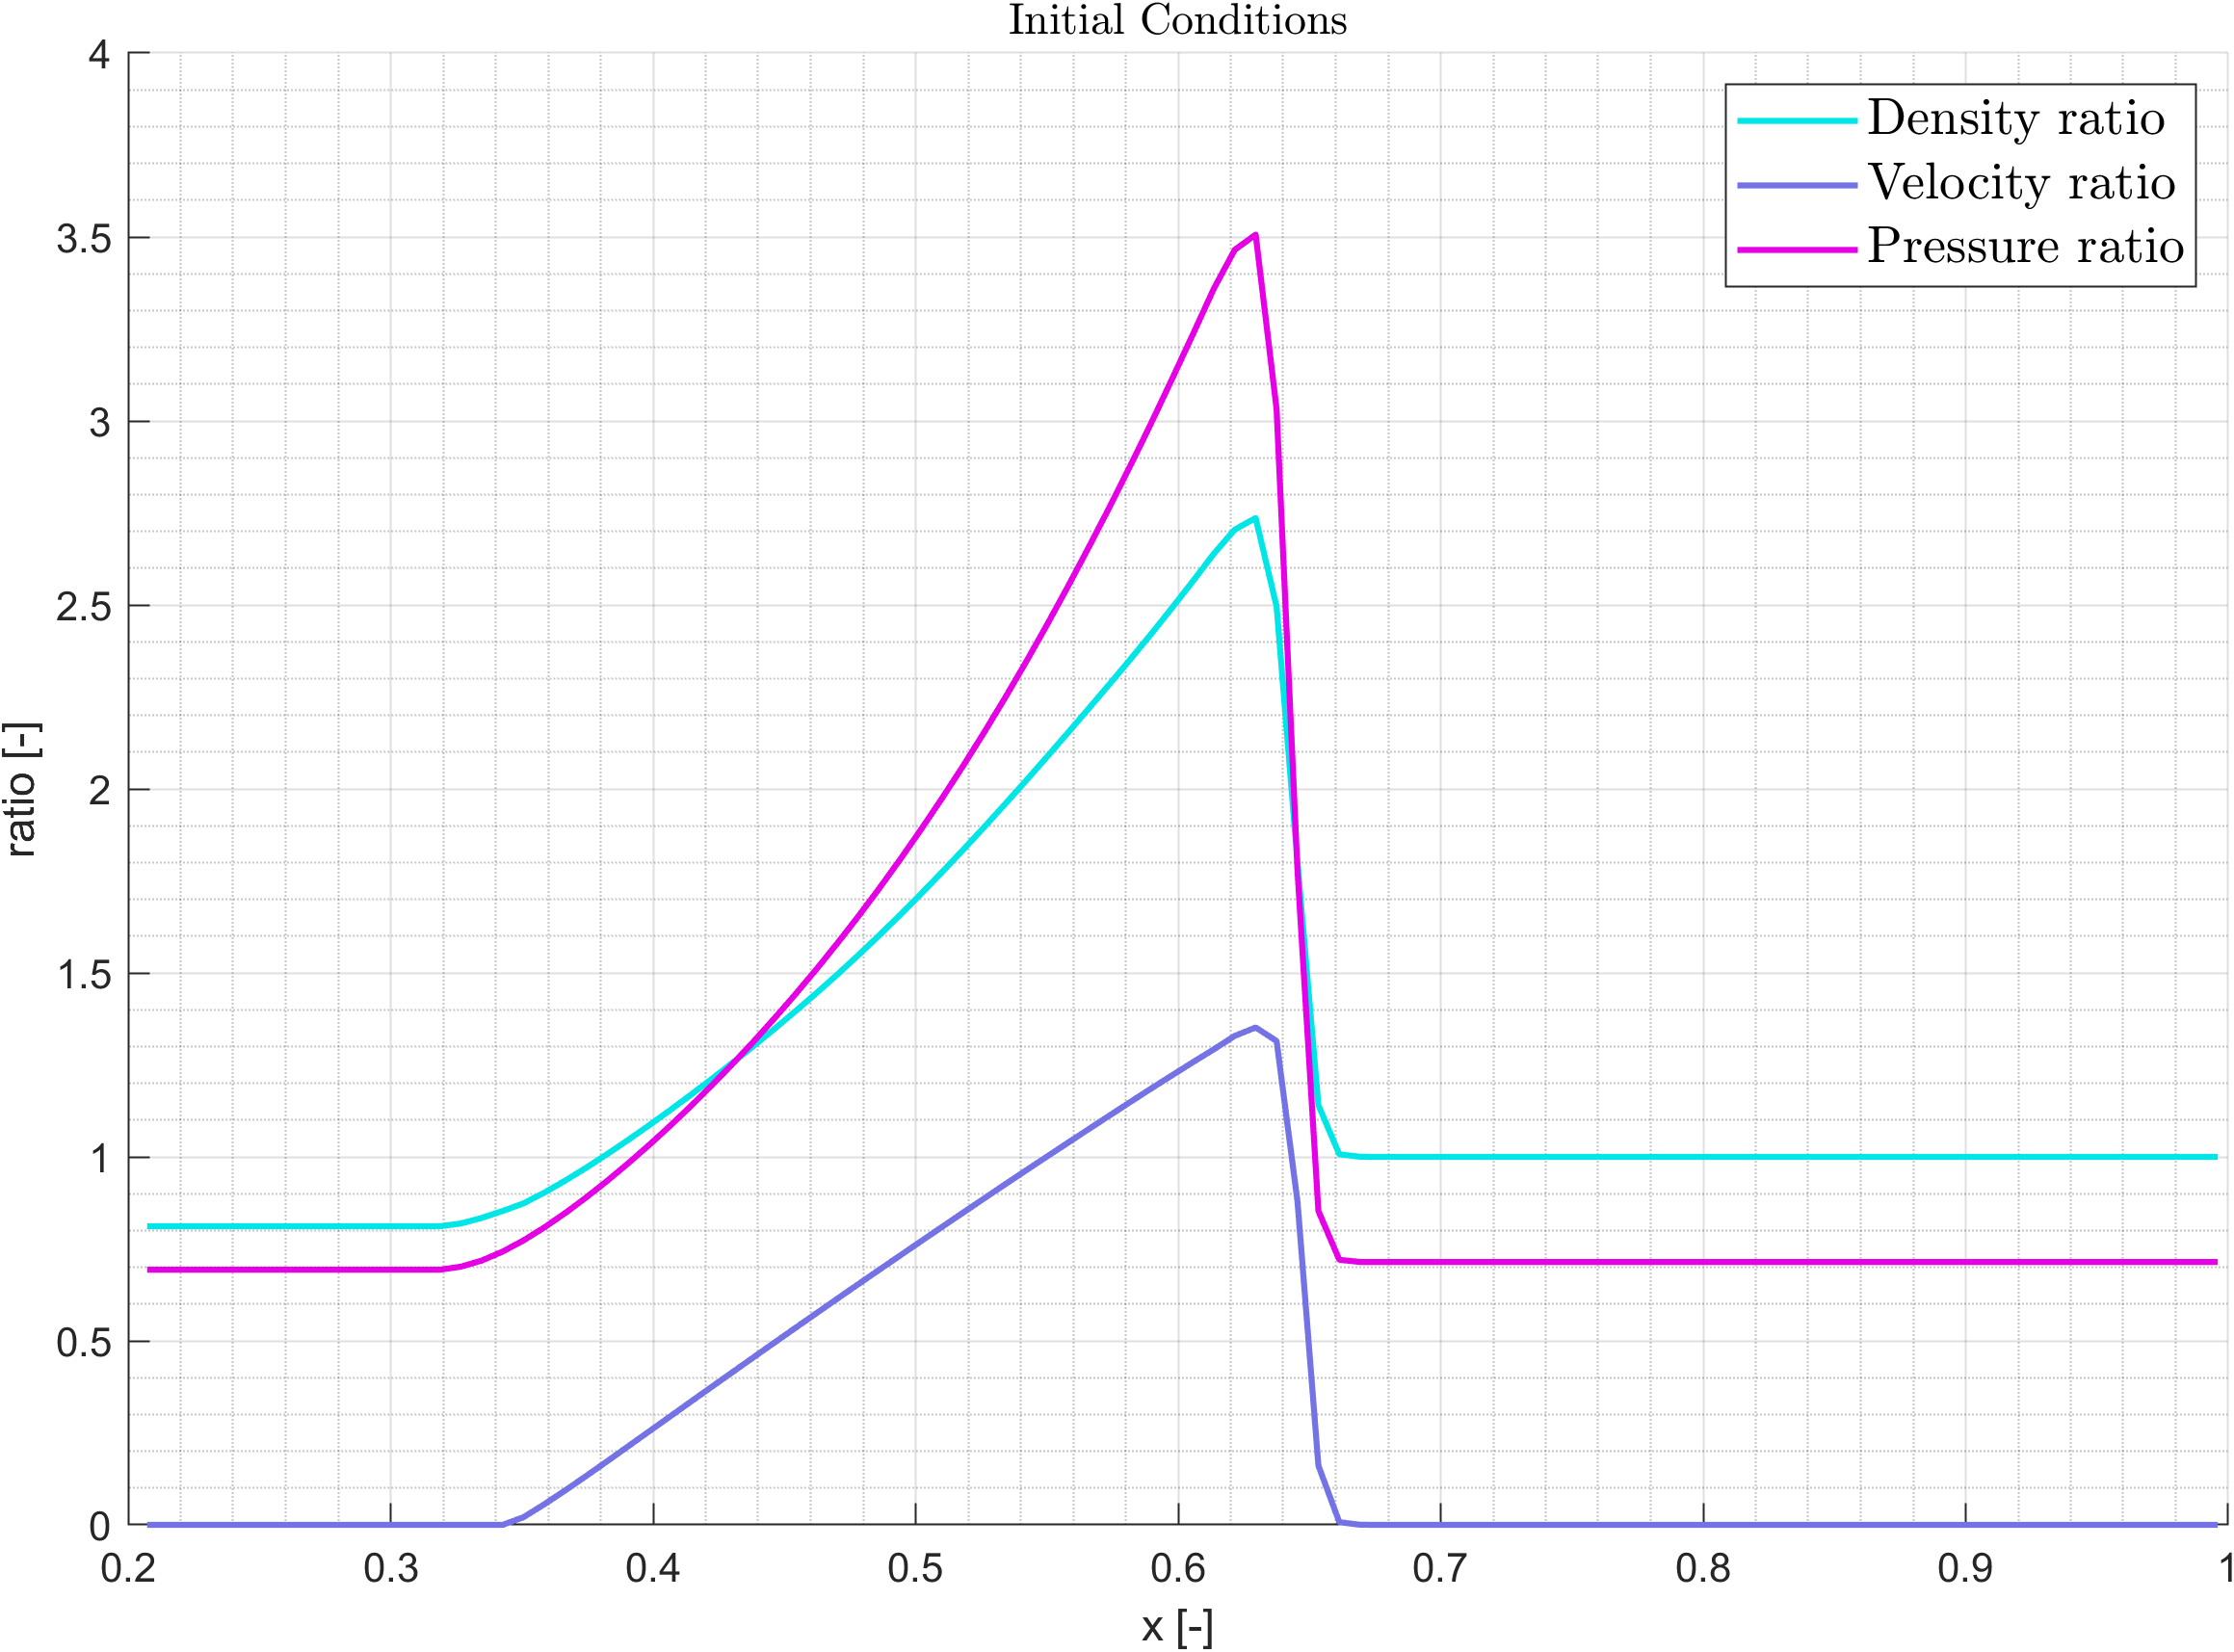
\includegraphics[width=0.4\textwidth]{images/Initial Conditions.png}
    \caption{Initial conditions}
    \label{fig: initial conditions}
\end{figure}

\subsection{Boundary Conditions}
On each side of the tube there is an adiabatic, solid wall boundary conditions. 
\begin{table}[H]
    \centering
    \begin{tabular}{cc||ccc||cc}
        $u_{\left(x=0.2\right)}=u_{\left(x=1.0\right)}=0$ &&& $\displaystyle\left.\frac{\partial p}{\partial x}\right|_{x=0.2}=\left.\frac{\partial p}{\partial x}\right|_{x=1.0}=0$ &&& $\displaystyle\left.\frac{\partial T}{\partial x}\right|_{x=0.2}=\left.\frac{\partial T}{\partial x}\right|_{x=1.0}=0$
    \end{tabular}
\end{table}

\section{Normalizing The Navier-Stokes Equations}
Since the initial conditions are normalized, there is a need to normalize the N-S equations. We will use the following normalizations:
\begin{equation}
    \begin{matrix}
        \rho=\rho_\infty\tilde{\rho}, & u=a_\infty\tilde{u}, & p=\gamma p_\infty\tilde{p}, & T=\gamma T_\infty\tilde{T}, & x=L\tilde{x}, & \displaystyle t=\frac{L}{a_\infty}\tilde{t}, & \mu=\mu_\infty\tilde{\mu}, & \kappa=\kappa_\infty\tilde{\kappa}
    \end{matrix}
\end{equation}
\nomenclature[F]{$\rho_\infty$}{density far away}
\nomenclature[F]{$a_\infty$}{speed of sound far away}
\nomenclature[F]{$p_\infty$}{pressure far away}
\nomenclature[F]{$T_\infty$}{temperature far away}
\nomenclature[F]{$\mu_\infty$}{coefficient of viscosity far away}
\nomenclature[F]{$\kappa_\infty$}{coefficient of thermal conductivity far away}

\noindent The normalization of the temperature was chosen to cancel out the $\gamma$ in the normalization of the pressure:
\begin{equation}
    \begin{array}{lcl}
        p & = & \rho RT \\
        \gamma p_\infty\tilde{p} & = & \rho_\infty\tilde{\rho}R\gamma T_\infty\tilde{T} \\
        \tilde{p} & = & \tilde{\rho}\tilde{T}
    \end{array}
\end{equation}
The pressure normalization can be written also as:
\begin{equation}
    p=\gamma p_\infty\tilde{p}=\gamma\rho_\infty RT_\infty\tilde{p}=\rho_\infty a_\infty^2\tilde{p}
    \label{eq: normalization for pressure}
\end{equation}
From equations \ref{eq: definitions} and \ref{eq: normalization for pressure} we can derive the normalization for the energy:
\begin{equation}
    \begin{array}{lcl}
        e & = & \displaystyle\frac{p}{\gamma-1}+\frac{1}{2}\rho u^2 \\\\
        e & = & \displaystyle\frac{\rho_\infty a_\infty^2\tilde{p}}{\gamma-1}+\frac{1}{2}\rho_\infty\tilde{\rho}a_\infty^2\tilde{a}^2 \\\\
        e & = & \displaystyle \rho_\infty a_\infty^2\left(\frac{\tilde{p}}{\gamma-1}+\frac{1}{2}\tilde{\rho}\tilde{a}^2\right) \\\\
        e & = & \rho_\infty a_\infty^2\tilde{e}
    \end{array}
\end{equation}
% The normalizations for $\mu$ and $\kappa$ are there for:
% \begin{equation}
%     \begin{matrix}
%         \begin{array}{lcl}
%             \tilde{\mu} & = & \displaystyle\frac{\mu}{\mu_\infty}
%         \end{array} & \begin{array}{lcl}
%             \tilde{\kappa} & = & \displaystyle\frac{\kappa}{\kappa_\infty}
%         \end{array}
%     \end{matrix}
% \end{equation}
After substituting the normalizations in the N-S equations we get:
\begin{equation}
    \parder{}{\displaystyle\frac{L}{a_\infty}\tilde{t}}\begin{pmatrix}
        \rho_\infty\tilde{\rho} \\\\
        \rho_\infty a_\infty\tilde{\rho}\tilde{u} \\\\
        \rho_\infty a_\infty^2\tilde{e}
    \end{pmatrix}+\parder{}{L\tilde{x}}\begin{pmatrix}
        \rho_\infty a_\infty\tilde{\rho}\tilde{u} \\\\
        \rho_\infty a_\infty^2\tilde{p}+\rho_\infty a_\infty^2\tilde{\rho}\tilde{u}^2 \\\\
        \rho_\infty a_\infty^3\left(\tilde{e}+\tilde{p}\right)\tilde{u}
    \end{pmatrix}=\parder{}{L\tilde{x}}\begin{pmatrix}
        0 \\\\
        \displaystyle\frac{4}{3}\mu_\infty a_\infty\tilde{\mu} \parder{\tilde{u}}{L\tilde{x}} \\\\
        \displaystyle\frac{4}{3}\mu_\infty a_\infty^2\tilde{\mu}\tilde{u}\parder{\tilde{u}}{L\tilde{x}}+\frac{\kappa_\infty a_\infty^2}{R}\tilde{\kappa}\parder{\tilde{T}}{L\tilde{x}}
    \end{pmatrix}
\end{equation}
Rearranging:
\begin{equation}
    \frac{\rho_\infty a_\infty}{L}\parder{}{\tilde{t}}\begin{pmatrix}
        \tilde{\rho} \\\\
        a_\infty\tilde{\rho}\tilde{u} \\\\
        a_\infty^2\tilde{e}
    \end{pmatrix}+\frac{\rho_\infty a_\infty}{L}\parder{}{\tilde{x}}\begin{pmatrix}
        \tilde{\rho}\tilde{u} \\\\
        a_\infty\tilde{p}+a_\infty\tilde{\rho}\tilde{u}^2 \\\\
        a_\infty^2\left(\tilde{e}+\tilde{p}\right)\tilde{u}
    \end{pmatrix}=\frac{\mu_\infty}{L^2}\parder{}{\tilde{x}}\begin{pmatrix}
        0 \\\\
        \displaystyle\frac{4}{3}a_\infty\tilde{\mu} \parder{\tilde{u}}{\tilde{x}} \\\\
        \displaystyle\frac{4}{3}a_\infty^2\tilde{\mu}\tilde{u}\parder{\tilde{u}}{\tilde{x}}+\frac{\kappa_\infty a_\infty^2}{\mu_\infty R}\tilde{\kappa}\parder{\tilde{T}}{\tilde{x}}
    \end{pmatrix}
\end{equation}
Dividing the second equation by $a_\infty$, the third equation by $a_\infty^2$, and the whole set of equations by $\displaystyle\frac{\rho_\infty a_\infty}{L}$ we get:
\begin{equation}
    \parder{}{\tilde{t}}\begin{pmatrix}
        \tilde{\rho} \\\\
        \tilde{\rho}\tilde{u} \\\\
        \tilde{e}
    \end{pmatrix}+\parder{}{\tilde{x}}\begin{pmatrix}
        \tilde{\rho}\tilde{u} \\\\
        \tilde{p}+\tilde{\rho}\tilde{u}^2 \\\\
        \left(\tilde{e}+\tilde{p}\right)\tilde{u}
    \end{pmatrix}=\frac{\mu_\infty}{L\rho_\infty a_\infty}\parder{}{\tilde{x}}\begin{pmatrix}
        0 \\\\
        \displaystyle\frac{4}{3}\tilde{\mu} \parder{\tilde{u}}{\tilde{x}} \\\\
        \displaystyle\frac{4}{3}\tilde{\mu}\tilde{u}\parder{\tilde{u}}{\tilde{x}}+\frac{\kappa_\infty}{\mu_\infty R}\tilde{\kappa}\parder{\tilde{T}}{\tilde{x}}
    \end{pmatrix}
\end{equation}
The Reynolds number and the mach number far away are defined as:
\begin{equation}
    \begin{array}{c}
        \begin{matrix}
            \displaystyle M_\infty=\frac{u_\infty}{a_\infty} & \displaystyle Re_{L\infty}=\frac{\rho_\infty u_\infty L}{\mu_\infty}
        \end{matrix} \\
        \Downarrow \\
        \displaystyle \frac{\mu_\infty}{L\rho_\infty a_\infty}=\frac{M_\infty}{Re_{L\infty}}
    \end{array}
\end{equation}
\nomenclature[F]{$M_\infty$}{mach number far away}
\nomenclature[N]{$Re_{L\infty}$}{Reynolds number with respect to L far away}
The Prandtl number far away is defined as:
\begin{equation}
    \begin{array}{c}
        \displaystyle Pr_\infty=\frac{c_p\mu_\infty}{\kappa_\infty} \\
        \Downarrow \\
        \displaystyle\frac{\kappa_\infty}{\mu_\infty R}=\frac{c_p}{Pr_\infty \left(c_p-c_v\right)}=\frac{\gamma}{Pr_\infty\left(\gamma-1\right)}
    \end{array}
\end{equation}
\nomenclature[N]{$Pr_\infty$}{Prandtl number far away}
Substituting into the normalized N-S equations:
\begin{equation}
    \parder{\tilde{Q}}{\tilde{t}}+\parder{\tilde{E}}{\tilde{x}}=\frac{M_\infty}{Re_{L\infty}}\parder{\tilde{E}_\nu}{\tilde{x}}
\end{equation}
Where:
\begin{equation}
    \begin{matrix}
        \tilde{Q}=\begin{pmatrix}
        \tilde{\rho} \\\\
        \tilde{\rho}\tilde{u} \\\\
        \tilde{e}
        \end{pmatrix}, & \tilde{E}=\begin{pmatrix}
        \tilde{\rho}\tilde{u} \\\\
        \tilde{p}+\tilde{\rho}\tilde{u}^2 \\\\
        \left(\tilde{e}+\tilde{p}\right)\tilde{u}
        \end{pmatrix}, & \tilde{E_\nu}=\begin{pmatrix}
        0 \\\\
        \displaystyle\frac{4}{3}\tilde{\mu} \parder{\tilde{u}}{\tilde{x}} \\\\
        \displaystyle\frac{4}{3}\tilde{\mu}\tilde{u}\parder{\tilde{u}}{\tilde{x}}+\frac{\gamma}{Pr_\infty\left(\gamma-1\right)}\tilde{\kappa}\parder{\tilde{T}}{\tilde{x}}
        \end{pmatrix}
    \end{matrix}
\end{equation}
The normalized Navier-Stokes equations are:
\begin{equation}
    \parder{\tilde{Q}}{\tilde{t}}+\parder{\tilde{E}}{\tilde{x}}=\frac{M_\infty}{Re_{L\infty}}\parder{\tilde{V}_1}{\tilde{x}}
\end{equation}
Where:
\begin{equation*}
    \tilde{V}_1=\tilde{V}_{1\left(\tilde{Q},\tilde{Q}_x\right)}=\tilde{E}_\nu
\end{equation*}

% \section{Linearizing The Navier-Stokes Equations In Time}
% To linearize the N-S equations we need to estimate the derivatives $\displaystyle\parder{\tilde{E}}{\tilde{x}}$ and $\displaystyle\parder{\tilde{V}_1}{\tilde{x}}$.

% \subsection{$\parder{\tilde{E}}{\tilde{x}}$ Estimation}
% \begin{equation}
%     \begin{array}{c}
%         \displaystyle\parder{\tilde{E}}{\tilde{x}}=\underbrace{\parder{\tilde{E}}{\tilde{Q}}}_{\tilde{A}}\parder{\tilde{Q}}{\tilde{x}} \\
%         \tilde{A}=\begin{pmatrix}
%             0 & 1 & 0 \\
%             \displaystyle\frac{\gamma-3}{2}\tilde{u}^2 & \left(3-\gamma\right)\tilde{u} & \gamma-1 \\
%             \displaystyle\left(\gamma-1\right)\tilde{u}^3\frac{\gamma\tilde{e}\tilde{u}}{\tilde{\rho}} & \displaystyle\frac{\gamma\tilde{e}}{\tilde{\rho}}-\frac{3\left(\gamma-1\right)\tilde{u}^2}{2} & \gamma\tilde{u}
%         \end{pmatrix}
%     \end{array}
% \end{equation}

% \subsection{$\parder{\tilde{V}_1}{\tilde{x}}$ Estimation}
% \begin{equation}
%     \begin{array}{c}
%         \displaystyle\parder{\tilde{V}_1}{\tilde{x}}=\underbrace{\parder{\tilde{V}_1}{\tilde{Q}}}_P\parder{\tilde{Q}}{\tilde{x}}+\underbrace{\parder{\tilde{V}_1}{\tilde{Q}_x}}_R\parder{\tilde{Q}_x}{\tilde{x}} \\\\
%         \displaystyle\parder{\tilde{V}_1}{\tilde{x}}=P\parder{\tilde{Q}}{\tilde{x}}+R\parder{\tilde{Q}_x}{\tilde{x}} \\\\
%     \end{array}
% \end{equation}
% \begin{equation}
%     \begin{array}{c}
%         \tilde{V}_1=V_{1\left(Q,Q_x\right)}
%     \end{array}
% \end{equation}

\section{The Computational Domain}
\subsection{Discretization}
The physical domain $\left[x_I,x_F\right]$ is discretized into N equispaced cells. The size of each cell is there for:
\begin{equation}
    \Delta x=\frac{x_F-x_I}{N}=\frac{L}{N}
\end{equation}
\nomenclature{$x_F$}{x coordinate of the end of the domain}
\nomenclature{$\Delta x$}{size of each cell in the domain}
\nomenclature{$L$}{characteristic length}
so the x coordinate of the i-th cell $x_i$ is:
\begin{equation}
    \begin{matrix}
        \displaystyle x_i=x_I+\frac{1}{2}\Delta x+\Delta x\cdot\left(i-1\right) && \text{when starting from $i=1$}
    \end{matrix}
\end{equation}
\nomenclature{$x_i$}{x coordinate of the i-th cell}

\subsection{Boundary Conditions}
In order to set the boundary conditions on the edge faces we will define ghost cells that will be calculated like so:
\begin{equation}
    \begin{array}{lcl}
        u_{\left(i=0\right)} &=& -u_{\left(i=1\right)} \\
        u_{\left(i=N+1\right)} &=& -u_{\left(i=N\right)}
    \end{array}
    \label{eq: velocity boundary}
\end{equation}
in order to maintain velocity zero on the boundary and like so:
\begin{equation}
    \begin{array}{lcl}
        T_{\left(i=0\right)} &=& T_{\left(i=1\right)} \\
        T_{\left(i=N+1\right)} &=& T_{\left(i=N\right)}
    \end{array}
    \label{eq: temp boundary}
\end{equation}
In order to maintain adiabatic boundary conditions.
Since the gradient of the pressure on the wall is zero, we get:
\begin{equation}
    \begin{array}{lcl}
        p_{\left(i=0\right)} &=& p_{\left(i=1\right)} \\
        p_{\left(i=N+1\right)} &=& p_{\left(i=N\right)}
    \end{array}
    \label{eq: pressure boundary}
\end{equation}
From equations \ref{eq: definitions}, \ref{eq: temp boundary}, and \ref{eq: pressure boundary} we can conclude:
\begin{equation}
    \begin{array}{lcl}
        \rho_{\left(i=0\right)} &=& \rho_{\left(i=1\right)} \\
        \rho_{\left(i=N+1\right)} &=& \rho_{\left(i=N\right)}
    \end{array}
    \label{eq: density boundary}
\end{equation}
and from equations \ref{eq: definitions}, \ref{eq: velocity boundary}, \ref{eq: pressure boundary}, and \ref{eq: density boundary} we can conclude:
\begin{equation}
    \begin{array}{lcl}
        e_{\left(i=0\right)} &=& e_{\left(i=1\right)} \\
        e_{\left(i=N+1\right)} &=& e_{\left(i=N\right)}
    \end{array}
    \label{eq: energy boundary}
\end{equation}

\section{The Numerical Schemes}
\subsection{Linearizing The Navier-Stokes Equations In Time}
\begin{equation}
    \begin{array}{lcl}
        \displaystyle\frac{\Delta Q}{\Delta t} & = & \displaystyle-\left(\parder{\tilde{E}}{\tilde{x}}-\parder{\tilde{V}_1}{\tilde{x}}\right)^{n+1} \\\\
        \displaystyle\frac{\Delta Q}{\Delta t} & = & \displaystyle-\left(\underbrace{\parder{\tilde{E}}{\tilde{Q}}}_{\tilde{A}}\parder{\tilde{Q}}{\tilde{x}}-\frac{M_\infty}{Re_{L\infty}}\left(\underbrace{\parder{\tilde{V}_1}{\tilde{Q}}}_{\tilde{P}}\parder{\tilde{Q}}{\tilde{x}}+\underbrace{\parder{\tilde{V}_1}{\tilde{Q}_x}}_{\tilde{R}}\parder{\tilde{Q}_x}{\tilde{x}}\right)\right)^{n+1}
    \end{array}
\end{equation}
Where:
\begin{equation}
    \begin{array}{ccl}
        \tilde{A} & = & \begin{pmatrix}
            0 & 1 & 0 \\
            \displaystyle\frac{\gamma-3}{2}\tilde{u}^2 & \left(3-\gamma\right)\tilde{u} & \gamma-1 \\
            \displaystyle-\frac{\gamma\tilde{e}\tilde{u}}{\tilde{\rho}}-\left(\gamma-1\right)\tilde{u}^3 & \displaystyle\frac{\gamma\tilde{e}}{\tilde{\rho}}-\frac{3\left(\gamma-1\right)\tilde{u}^2}{2} & \gamma\tilde{u}
        \end{pmatrix} \\\\
        \tilde{P}-\tilde{R}_x & = & \displaystyle-\frac{1}{\rho}\begin{pmatrix}
            0 & 0 & 0 \\\\
            \displaystyle-\tilde{u}\left(\frac{4}{3}\tilde{\mu}\right)_x & \displaystyle\left(\frac{4}{3}\tilde{\mu}\right)_x & 0 \\\\
            \displaystyle-\tilde{u}^2\left(\frac{4}{3}\tilde{\mu}\right)_x & \displaystyle\tilde{u}\left(\frac{4}{3}\tilde{\mu}\right)_x & 0
        \end{pmatrix} \\\\
        \tilde{R} & = & \displaystyle-\frac{1}{\rho}\begin{pmatrix}
            0 & 0 & 0 \\\\
            \displaystyle\frac{4}{3}\tilde{u}\tilde{\mu} & \displaystyle-\frac{4}{3}\tilde{\mu} & 0 \\\\
            \displaystyle\left(\frac{4}{3}\tilde{\mu}-\textcolor{blue}{\alpha}\frac{\tilde{\kappa}}{c_v}\right)\tilde{u}^2+\textcolor{blue}{\alpha}\frac{\tilde{\kappa}}{c_v}\frac{\tilde{e}}{\tilde{\rho}} & \displaystyle-\left(\frac{4}{3}\tilde{\mu}-\textcolor{blue}{\alpha}\frac{\tilde{\kappa}}{c_v}\right)\tilde{u} & \displaystyle-\textcolor{blue}{\alpha}\frac{\tilde{\kappa}}{c_v}
        \end{pmatrix}
    \end{array}
\end{equation}
and $\textcolor{blue}{\alpha}$ is: $$\textcolor{blue}{\alpha=\frac{\gamma}{Pr_\infty\left(\gamma-1\right)}}$$

\subsection{First Order Approximate Riemann Roe Method}

\subsection{First Order Steger-Warming -- Explicit}
A is a Diagonalizable matrix and can be written as:
\begin{equation}
    \begin{array}{c}
        \tilde{A}=\tilde{T}\tilde{\Lambda}\tilde{T}^{-1} \\
        \tilde{T}=\begin{pmatrix}
            1 & \displaystyle\frac{\tilde{\rho}}{2\tilde{a}} & \displaystyle-\frac{\tilde{\rho}}{2\tilde{a}} \\\\
            \tilde{u} & \displaystyle\frac{\tilde{\rho}}{2\tilde{a}}\left(\tilde{u}+\tilde{a}\right) & \displaystyle-\frac{\tilde{\rho}}{2\tilde{a}}\left(\tilde{u}-\tilde{a}\right) \\\\
            \displaystyle\frac{\tilde{u}^2}{2} & \displaystyle\frac{\tilde{\rho}}{2\tilde{a}}\left(\frac{\tilde{u}^2}{2}+\tilde{u}\tilde{a}+\frac{\tilde{a}^2}{\gamma-1}\right) & \displaystyle-\frac{\tilde{\rho}}{2\tilde{a}}\left(\frac{\tilde{u}^2}{2}-\tilde{u}\tilde{a}+\frac{\tilde{a}^2}{\gamma-1}\right)
        \end{pmatrix} \\\\
        \tilde{\Lambda}=\begin{pmatrix}
            \tilde{u} & 0 & 0 \\
            0 & \tilde{u}+\tilde{a} & 0 \\
            0 & 0 & \tilde{u}-\tilde{a}
        \end{pmatrix} \\\\
        \tilde{T}^{-1}=\begin{pmatrix}
            \displaystyle1-\frac{\gamma-1}{2}\frac{\tilde{u}^2}{\tilde{a}^2} & \displaystyle\left(\gamma-1\right)\frac{\tilde{u}^2}{\tilde{a}^2} & -\frac{\gamma-1}{\tilde{a}^2} \\\\
            \displaystyle\frac{1}{\tilde{\rho}\tilde{a}}\left(\left(\gamma-1\right)\tilde{u}^2-\tilde{u}\tilde{a}\right) & \displaystyle\frac{1}{\tilde{\rho}\tilde{a}}\left(\tilde{a}-\left(\gamma-1\right)\tilde{u}\right) & \displaystyle\frac{\gamma-1}{\tilde{\rho}\tilde{a}} \\\\
            \displaystyle-\frac{1}{\tilde{\rho}\tilde{a}}\left(\left(\gamma-1\right)\tilde{u}^2+\tilde{u}\tilde{a}\right) & \displaystyle\frac{1}{\tilde{\rho}\tilde{a}}\left(\tilde{a}+\left(\gamma-1\right)\tilde{u}\right) & \displaystyle-\frac{\gamma-1}{\tilde{\rho}\tilde{a}}
        \end{pmatrix}
    \end{array}
\end{equation}
Where:
\begin{equation*}
    \tilde{a}=\sqrt{\frac{\gamma\tilde{p}}{\tilde{\rho}}}
\end{equation*}
Let the $\Lambda^\pm$ matrix be defined as:
\begin{equation}
    \tilde{\Lambda}^\pm=\begin{pmatrix}
        \displaystyle\frac{\tilde{u}\pm\left|\tilde{u}\right|}{2} & 0 & 0 \\
        0 & \displaystyle\frac{\tilde{u}+\tilde{a}\pm\left|\tilde{u}+\tilde{a}\right|}{2} & 0 \\
        0 & 0 & \displaystyle\frac{\tilde{u}-\tilde{a}\pm\left|\tilde{u}-\tilde{a}\right|}{2}
    \end{pmatrix}
\end{equation}
Where the matrix $\tilde{\Lambda}^+$ contains only positive eigenvalues and the matrix $\tilde{\Lambda}^-$ contains only negative eigenvalues. \\ Define:
\begin{equation}
    \begin{matrix}
        \begin{array}{ccl}
            \tilde{A}^+ & \triangleq & \tilde{T}\tilde{\Lambda}^+\tilde{T}^{-1} \\
            \tilde{A}^- & \triangleq & \tilde{T}\tilde{\Lambda}^-\tilde{T}^{-1}
        \end{array} & \Rightarrow & \begin{array}{ccl}
            \tilde{A} & = & \tilde{A}^++\tilde{A}^- \\
            \left|\tilde{A}\right| & \triangleq & \tilde{A}^+-\tilde{A}^-
        \end{array}
    \end{matrix}
\end{equation}
Assuming a perfect gas, the flux vector $\tilde{E}_{\left(Q\right)}$ is a homogeneous function of degree one in $\tilde{Q}$, meaning:$$\forall\alpha\ \ \ \ \tilde{E}_{\left(\alpha \tilde{Q}\right)}=\alpha \tilde{E}_{\left(\tilde{Q}\right)}$$The homogeneity allows to rewrite the flux vector $\tilde{E}$ as:
\begin{equation}
    \tilde{E}=\tilde{A}\tilde{Q}=\left(\tilde{A}^++\tilde{A}^-\right)\tilde{Q}=\underbrace{\tilde{A}^+\tilde{Q}}_{\tilde{E}^+}+\underbrace{\tilde{A}^-\tilde{Q}}_{\tilde{E}^-}=\tilde{E}^++\tilde{E}^-
\end{equation} 
There is a discontinuities and deference between $\tilde{E}^+,\tilde{E}^-$.
% There is a discontinuities and deference between $\tilde{E}^+,\tilde{E}^-$ for example:
% \begin{equation}
%     \begin{matrix}
%         \tilde{E}^+_1=\left\{\begin{array}{lc}
%             0 & M\le-1 \\\\
%             \displaystyle\frac{\tilde{\rho} \tilde{a}}{2\gamma}\left(M+1\right) & -1\le M\le0 \\\\
%             \displaystyle\frac{\tilde{\rho} \tilde{a}}{2\gamma}\left(\left(2\gamma-1\right)M+1\right) & 0\le M\le1 \\\\
%             \tilde{E}_1 & 1\le M
%         \end{array}\right. & \tilde{E}^-_1=\left\{\begin{array}{lc}
%             \tilde{E}_1 & M\le-1 \\\\
%             \displaystyle\frac{\tilde{\rho} \tilde{a}}{2\gamma}\left(\left(2\gamma-1\right)M-1\right) & -1\le M\le0 \\\\
%             \displaystyle\frac{\tilde{\rho} \tilde{a}}{2\gamma}\left(M-1\right) & 0\le M\le1 \\\\
%             0 & 1\le M
%         \end{array}\right.
%     \end{matrix}
% \end{equation}
To eliminate the discontinuities and guarantee a smooth transition through critical points (sonic points or stagnation points), a blending function is introduced together with a blending parameter $\varepsilon$. An appropriate choice of the blending parameter has to be chosen.
\begin{equation}
    \begin{matrix}
        \begin{array}{lcl}
            \tilde{\lambda}^+ & = & \displaystyle\frac{\tilde{\lambda}+\left|\tilde{\lambda}\right|}{2} \\\\
            \tilde{\lambda}^- & = & \displaystyle\frac{\tilde{\lambda}-\left|\tilde{\lambda}\right|}{2}
        \end{array} & \Rightarrow & \begin{array}{lcl}
            \tilde{\lambda}^{+'} & = & \displaystyle\frac{\tilde{\lambda}+\sqrt{\tilde{\lambda}^2+\varepsilon^2}}{2} \\\\
            \tilde{\lambda}^{-'} & = & \displaystyle\frac{\tilde{\lambda}-\sqrt{\tilde{\lambda}^2+\varepsilon^2}}{2}
        \end{array}
    \end{matrix}
\end{equation}
Rewriting the conservation law from of the N-S equations:
\begin{equation}
    \parder{\tilde{Q}}{\tilde{t}}=-\parder{\tilde{E}^+}{\tilde{x}}-\parder{\tilde{E}^-}{\tilde{x}}+\frac{M_\infty}{Re_{L\infty}}\parder{\tilde{V}_1}{\tilde{x}}
\end{equation}
A simple, explicit, first order (in space and time) scheme is obtained using:
\begin{equation}
    \Delta\tilde{Q}_i^n=-\frac{\Delta\tilde{t}}{\Delta\tilde{x}}\left(\nabla\tilde{E}_i^{+n}+\Delta\tilde{E}_i^{-n}+\frac{M_\infty}{Re_{L\infty}}\colorbox{red}{WTF TO DO?}\right)
\end{equation}
And advancing the solution by:
\begin{equation}
    \tilde{Q}_i^{n+1}=\Delta\tilde{Q}_i^n+\tilde{Q}_i^n
\end{equation} 

\subsection{First Order Steger-Warming -- Implicit}

\end{document}